\documentclass[conference]{IEEEtran}
\IEEEoverridecommandlockouts

\usepackage{cite}
\usepackage{amsmath,amssymb,amsfonts}
\usepackage{algorithm}
\usepackage{algpseudocode}
\usepackage{graphicx}
\usepackage{booktabs}
\usepackage{xcolor}
\usepackage{tikz}
\usetikzlibrary{arrows.meta,positioning,calc,fit,backgrounds,shapes.geometric}
\usepackage{pgfplots}
\pgfplotsset{compat=1.18}
\usepgfplotslibrary{groupplots}
\usepackage[hidelinks]{hyperref}
\usepackage{url}

% ---- shared scientific plot style (consistent palette across figures) ----
\definecolor{cRules}{RGB}{84,110,135}    % slate (deterministic baseline)
\definecolor{cSdk}{RGB}{211,94,49}       % warm orange (agentic engine)
\definecolor{cTier1}{RGB}{173,196,214}   % rule tier
\definecolor{cTier2}{RGB}{93,140,166}    % embedding tier
\definecolor{cTier3}{RGB}{211,94,49}     % llm tier
\pgfplotsset{
  scilabel/.style={font=\scriptsize},
  every axis/.append style={
    line width=0.5pt, tick align=outside, tick style={black},
    label style={font=\scriptsize}, tick label style={font=\scriptsize},
    legend style={font=\scriptsize, draw=none, fill=none},
    title style={font=\scriptsize\bfseries},
    axis line style={-},
  },
}

% Compact code style for inline tool signatures
\newcommand{\code}[1]{\texttt{\small #1}}

\definecolor{boxblue}{RGB}{225,235,250}
\definecolor{boxgreen}{RGB}{224,242,228}
\definecolor{boxgray}{RGB}{238,238,238}
\definecolor{boxorange}{RGB}{252,238,220}

\begin{document}

\title{A Hybrid Agentic Architecture for Autonomous LLM-Security Threat-Intelligence Collection over Live Vulnerability Sources}

\author{\IEEEauthorblockN{Anonymous Author(s)}
\IEEEauthorblockA{\textit{Affiliation withheld for review} \\
\textit{Contact withheld}}
}

\maketitle

\begin{abstract}
The security of large language model (LLM) applications is a fast-moving target whose evidence is scattered across heterogeneous public feeds: the National Vulnerability Database (NVD), the CISA Known Exploited Vulnerabilities (KEV) catalog, the OSV.dev open-source advisory database, and the arXiv research corpus. Existing collection pipelines query these sources with fixed templates, a fixed source rotation, and a fixed number of rounds, leaving the genuinely hard decisions---\emph{which source to query, what to search for, which advanced operators to use, and when to stop}---hard-coded rather than reasoned about. We present the architecture of an autonomous intelligence-collection agent that delegates exactly these four decisions to an LLM operating inside a native tool-use loop, while a deterministic Python controller retains the round skeleton, budget safety valves, and persistence. The design rests on four ideas: (i) a \emph{hybrid controller} in which every LLM decision is a structured, tool-forced call that falls back to a shared deterministic rule on any failure, so behavior never drops below a verified baseline; (ii) four \emph{typed source tools} exposed through an in-process MCP server that surface each feed's advanced query operators directly to the agent; (iii) a \emph{UCB1 multi-armed bandit} that recommends sources from accumulated per-source yield while leaving the final choice to the agent; and (iv) a \emph{three-tier relevance filter} (rule, embedding, flash-LLM) and a compact context digest that keep the decision loop cheap and auditable. We describe the engine-factory abstraction that lets a deterministic and an agentic engine share one rule implementation, a \emph{coverage-first} termination policy in which a depth-quota coverage gate and a marginal-information stall detector bound the LLM stop decision, and a same-budget A/B evaluation over nine frozen LLM-security collection goals (two of them multi-topic), each engine run three times per goal on live sources. The results reframe \emph{when} autonomy pays. On the primary objective---completeness of target-topic coverage to a depth quota---the agentic engine reaches full coverage on six of nine goals versus four for the well-tuned deterministic baseline, is never lower on any goal, and lifts mean coverage from $0.69$ to $0.95$ ($+38\%$), closing sparse gaps the fixed policy never reaches (e.g.\ agent-tool-abuse: $1.00$ vs $0.00$). This costs per-call efficiency: averaged over goals the agent is $8\%$ lower on relevant-items-per-call because it spends calls chasing sparse topics, while retrieving $60\%$ more items per call and terminating at the hindsight-optimal round on all nine goals (versus a mean one-fifth-round overshoot for the baseline), at $97.7\%$ live structured-decision reliability. We argue this coverage--efficiency trade-off---made explicitly tunable by the coverage gate---is the honest characterization of when an agentic collector earns its cost.
\end{abstract}

\begin{IEEEkeywords}
LLM security, threat intelligence, autonomous agents, tool use, multi-armed bandits, cyber threat intelligence, agentic systems
\end{IEEEkeywords}

\section{Introduction}

Large language models are now embedded in production software as chat assistants, retrieval-augmented applications, and tool-using agents. This deployment surface has produced a distinct class of vulnerabilities---prompt injection, jailbreaks, retrieval-augmented generation (RAG) poisoning, agent tool abuse, AI data leakage, and model-supply-chain compromise---codified in community taxonomies such as the OWASP Top~10 for LLM Applications~\cite{owasp2025llmtop10} and demonstrated in the wild~\cite{greshake2023injection}. Unlike a single CVE feed, the evidence for these threats is fragmented: a newly exploited deserialization bug in a model server appears first in NVD~\cite{nvd} and the CISA KEV catalog~\cite{cisakev}; an affected Python package surfaces in OSV.dev~\cite{osv}; and the attack technique itself is often described weeks earlier in an arXiv preprint~\cite{arxivapi}. An effective LLM-security intelligence pipeline must therefore continuously harvest, cross-reference, and prioritize across all of these.

Automating this harvest is more than a crawling problem. Each source has its own retrieval semantics and a rich set of advanced operators---NVD exposes CWE filtering, CVSS-severity thresholds, publication-date windows, and a KEV flag; arXiv accepts a boolean field-scoped query language with category restrictions; OSV is package-centric (ecosystem, package name, purl); CISA KEV matches product and vulnerability-type tokens. The collection task is a sequence of decisions: \emph{which sources to query this round}, \emph{what query text and operators to use}, and \emph{whether the marginal yield justifies another round}. In most pipelines, including the deterministic baseline we build upon, these decisions are made by hand-tuned rules: a fixed action sequence, template queries built from a topic$\rightarrow$terms table, a round-robin over operators, and a stop condition driven by a coverage threshold. The signals needed to decide better---per-round novelty, duplicate ratio, noise ratio, per-source yield, open coverage gaps---are already recorded, but they are never shown to a reasoner.

This paper presents the architecture of an autonomous collection agent that closes that gap. The agent runs inside a native tool-use loop provided by the Claude Agent SDK~\cite{claudeagentsdk} and takes over four decisions---source selection, query formulation, advanced-operator use, and termination---grounding each in a compact digest of the recorded metrics. Crucially, the agent does not replace the controller. A Python controller keeps the round skeleton, enforces budgets through hooks, and owns persistence; every agent decision is a structured tool-forced call validated against a Pydantic schema, and any failure---timeout, parse error, validation error, or runtime unavailability---falls back to the \emph{same} deterministic rule the baseline engine uses. The result is an engine whose floor is a verified rule-based system and whose ceiling is autonomous, multi-step reasoning.

\noindent\textbf{Contributions.} We make the following architectural contributions:
\begin{itemize}
  \item A \emph{hybrid controller} pattern (Section~\ref{sec:overview}--\ref{sec:decisions}) in which an agentic engine and a deterministic engine share one rule module, selected by an engine factory, with a three-layer fallback (decision / round / engine) that renders every degradation observable rather than silent.
  \item A \emph{typed source-tool layer} (Section~\ref{sec:tools}) that wraps four live sources as in-process MCP tools whose typed parameters expose advanced operators directly to the agent, with descriptions that teach effective operator combinations.
  \item A \emph{bandit-informed source-selection} mechanism (Section~\ref{sec:bandit}) and a \emph{three-tier relevance filter} (Section~\ref{sec:relevance}) that together turn raw collection counts into a trustworthy yield signal and a per-topic coverage measurement, plus a context-engineering discipline (Section~\ref{sec:context}) that feeds summaries, never raw documents, to the decision loop.
  \item A \emph{coverage-first termination policy} (Section~\ref{sec:decisions}) that makes completeness a hard constraint: a depth-quota coverage gate forbids stopping while a target topic is under-covered, a marginal-information stall detector prevents futile loops on unreachable topics, and both bound---rather than replace---the LLM stop decision under a strict priority order.
  \item A completed nine-goal \emph{same-budget A/B evaluation} (Section~\ref{sec:eval}) that makes the ``intelligence gain'' falsifiable, reporting coverage completeness as the primary metric alongside efficiency, volume, and reliability.
\end{itemize}

The emphasis of this paper is architecture, but we back it with a completed same-budget A/B study (Section~\ref{sec:eval}) over nine frozen goals, two of them multi-topic. We report the outcome without cherry-picking: where the deterministic baseline wins on per-call efficiency, we say so, and we trace the agentic engine's coverage advantage to the specific mechanisms that produce it.

\section{Background and Related Work}

\textbf{Cyber threat intelligence (CTI) automation.} Structured CTI exchange formats such as STIX~\cite{stix} and adversary-behavior knowledge bases such as MITRE ATT\&CK~\cite{strom2018attack} standardize \emph{what} intelligence looks like once collected, but say little about the active, multi-source \emph{acquisition} loop. Recent work applies LLMs to CTI knowledge-graph construction under data scarcity~\cite{cheng2024ctinexus}; our system consumes such extractors downstream but the collection engine described here is upstream and independent of them.

\textbf{LLM agents and tool use.} The ReAct paradigm~\cite{yao2023react} interleaves reasoning traces with tool actions, and Toolformer~\cite{schick2023toolformer} shows models can learn to call APIs; chain-of-thought prompting~\cite{wei2022cot} underpins the multi-step decisions we elicit. The Model Context Protocol (MCP)~\cite{anthropicmcp} standardizes how tools are exposed to an agent, and the Claude Agent SDK~\cite{claudeagentsdk} provides a native tool loop, in-process MCP servers, and lifecycle hooks. We use these mechanisms not as an end-to-end autonomous crawler but as the substrate for a tightly bounded set of decisions.

\textbf{Source selection as a bandit problem.} Choosing which feed to query under a fixed budget is naturally an exploration--exploitation problem. We adopt UCB1~\cite{auer2002ucb}, whose finite-time regret guarantees and parameter-free form suit a cold-start setting with sparse per-source reward history~\cite{lattimore2020bandit}. Unlike a pure bandit controller, we treat the bandit as an \emph{advisor}: its ranking is rendered into the agent's context and may be overridden with a rationale.

\textbf{Relevance filtering.} Tiered filtering---cheap lexical rules first, dense-embedding similarity~\cite{karpukhin2020dpr} next, an LLM judge last---lets us spend model calls only on genuinely ambiguous items. This ``cheapest-first'' cascade is the relevance analogue of staged retrieval and keeps the noise signal that drives both bandit reward and termination trustworthy.

\section{System Overview}
\label{sec:overview}

\subsection{Design principle: a hybrid controller}

The central architectural decision is that the LLM does \emph{not} own the loop. Figure~\ref{fig:arch} shows the layered design. A Python controller owns four things the agent must never be trusted with: the round skeleton, the API-call budget and its safety valves, blackboard accounting, and persistence. The agent owns one thing: the decisions that benefit from reasoning over context. The two engines---a deterministic \emph{rules} engine (\code{RealIntelRunController}) and an agentic \emph{sdk} engine (\code{SdkIntelRunController})---are interchangeable behind a factory:

\begin{quote}
\code{create\_intel\_controller(...)} reads \code{INTEL\_ENGINE}\\ $\in\{$\code{rules}, \code{sdk}$\}$, probes runtime availability, and returns the agentic controller only when both the SDK package and a provider key are present; otherwise it transparently returns the rules controller.
\end{quote}

This factory is the outermost of three fallback layers (Section~\ref{sec:context}). Because both engines emit the identical blackboard schema, run-file layout, and \code{real-} run-id prefix, every downstream consumer---the web console, the knowledge-graph adapter, and the evaluation harness---is engine-agnostic.

\begin{figure}[t]
\centering
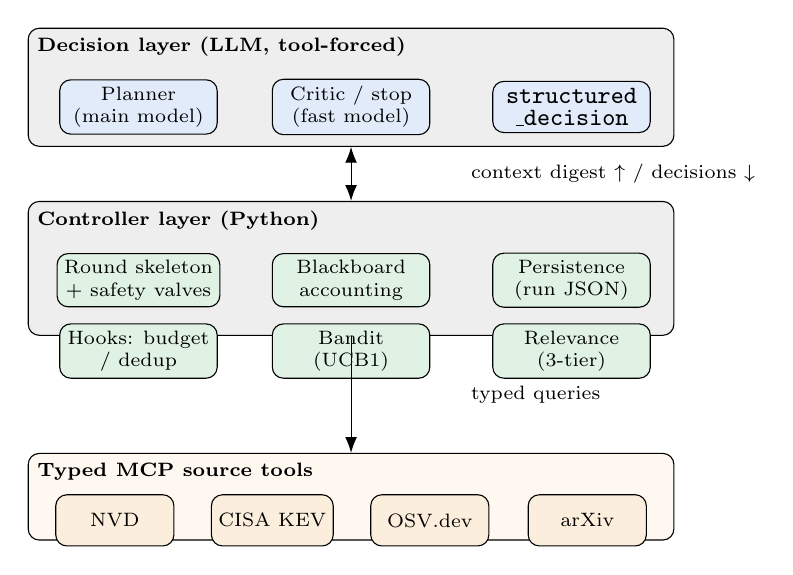
\begin{tikzpicture}[
  font=\scriptsize,
  box/.style={draw, rounded corners, align=center, minimum height=6.5mm, inner sep=2.5pt},
  lay/.style={draw, rounded corners, align=center, fill=boxgray, minimum width=82mm, inner sep=3pt},
  ag/.style={box, fill=boxblue, minimum width=20mm},
  ct/.style={box, fill=boxgreen, minimum width=20mm},
  src/.style={box, fill=boxorange, minimum width=15mm},
  >={Latex[length=2mm]}
]
% Agent layer
\node[lay, minimum height=15mm] (alayer) at (0,3.0) {};
\node[anchor=north west, font=\scriptsize\bfseries] at (alayer.north west) {Decision layer (LLM, tool-forced)};
\node[ag] (plan) at (-2.7,2.75) {Planner\\(main model)};
\node[ag] (crit) at (0.0,2.75) {Critic / stop\\(fast model)};
\node[ag] (sd)   at (2.8,2.75) {\code{structured}\\\code{\_decision}};

% Controller layer
\node[lay, minimum height=17mm] (clayer) at (0,0.7) {};
\node[anchor=north west, font=\scriptsize\bfseries] at (clayer.north west) {Controller layer (Python)};
\node[ct] (skel) at (-2.7,0.55) {Round skeleton\\+ safety valves};
\node[ct] (bb)   at (0.0,0.55) {Blackboard\\accounting};
\node[ct] (pers) at (2.8,0.55) {Persistence\\(run JSON)};
\node[ct, minimum width=20mm] (hooks) at (-2.7,-0.35) {Hooks: budget\\/ dedup};
\node[ct, minimum width=20mm] (band) at (0.0,-0.35) {Bandit\\(UCB1)};
\node[ct, minimum width=20mm] (rel) at (2.8,-0.35) {Relevance\\(3-tier)};

% Tool + source layer
\node[lay, minimum height=11mm, fill=boxorange!40] (tlayer) at (0,-2.2) {};
\node[anchor=north west, font=\scriptsize\bfseries] at (tlayer.north west) {Typed MCP source tools};
\node[src] (nvd) at (-3.0,-2.5) {NVD};
\node[src] (kev) at (-1.0,-2.5) {CISA KEV};
\node[src] (osv) at (1.0,-2.5) {OSV.dev};
\node[src] (arx) at (3.0,-2.5) {arXiv};

\draw[<->] (alayer) -- (clayer) node[midway,right,xshift=14mm,yshift=0pt]{context digest $\uparrow$ / decisions $\downarrow$};
\draw[->] (clayer) -- (tlayer) node[midway,right,xshift=14mm]{typed queries};
\end{tikzpicture}
\caption{Layered hybrid architecture. The LLM decision layer reasons over a compact context digest and returns tool-forced structured decisions; the Python controller layer owns the loop, budget hooks, bandit, relevance filter, accounting, and persistence; the four live sources are exposed as typed in-process MCP tools.}
\label{fig:arch}
\end{figure}

\subsection{The blackboard and the round skeleton}

State lives on a single \code{IntelRunBlackboard}: approved sources, accumulated \code{raw\_items}, a \code{query\_history} (one entry per round recording \code{novelty\_score}, \code{noise\_ratio}, \code{duplicate\_ratio}, and per-source plans), \code{coverage\_gaps}, \code{reflection\_notes}, a \code{RunBudget} (max rounds, max API calls, max sources), and run \code{metrics}. The controller iterates rounds up to \code{max\_rounds}; within each round it (1)~renders a context digest, (2)~selects sources, (3)~plans source-specific queries, (4)~enforces the call budget, (5)~executes queries and merges the batch (deduplicating against prior items and computing the per-round metrics), (6)~runs relevance annotation and coverage analysis, and (7)~decides whether to continue. Steps~2,~3, and~7 are the agentic decision points; the rest are deterministic bookkeeping shared verbatim with the rules engine via \code{intel/rules.py}.

\section{Autonomous Decision Architecture}
\label{sec:decisions}

\subsection{From seven hard-coded decisions to four reasoned ones}

The deterministic baseline contains seven decision points (action selection, yield assessment, coverage analysis, semantic expansion, strategy rewrite, completeness, and source-query construction), each implemented as a pure function in \code{intel/rules.py}. The agentic engine elevates four of these---the ones where reasoning over context pays off---to LLM decisions, and keeps the rest as deterministic post-processing. Table~\ref{tab:decisions} maps each autonomous capability to its structured output schema and its rule fallback.

\begin{table}[t]
\centering
\caption{The four autonomous decisions, their structured output schemas, and the deterministic fallback invoked on any failure.}
\label{tab:decisions}
\renewcommand{\arraystretch}{1.25}
\begin{tabular}{@{}p{1.55cm}p{2.45cm}p{3.0cm}@{}}
\toprule
\textbf{Capability} & \textbf{Output schema} & \textbf{Deterministic fallback} \\
\midrule
Source selection & \code{SourceSelection-} \code{Decision} & bandit top-$k$ ranking executed directly \\
Query \& operators & \code{CollectionPlan-} \code{Decision} (per-source proposals) & \code{build\_source\_query\_specs} (template + rotation) \\
Query rewrite & \code{RewriteDecision-} \code{Output} & \code{fallback\_rewrite\_} \code{decision} (gap-driven) \\
Termination & \code{Completeness-} \code{DecisionOutput} & coverage / yield / budget rule \\
\bottomrule
\end{tabular}
\end{table}

\subsection{The structured-decision engine}

Every decision flows through one mechanism, \code{StructuredDecisionEngine.decide}, which preserves the baseline's contract---``agent output preferred, deterministic rule as backstop''---while making failures countable. Given a decision name, a prompt, and a Pydantic output model, it:

\begin{enumerate}
  \item converts the Pydantic model to a JSON schema (inlining \code{\$defs} so nested proposal lists remain valid MCP tool inputs);
  \item issues a \emph{tool-forced} query: a single ephemeral MCP tool \code{submit\_decision} is registered with that schema, and the prompt instructs the model to call it exactly once. Tool forcing proved more reliable across Anthropic-compatible endpoints than native structured-output modes (Section~\ref{sec:eval});
  \item captures the tool input, or, defensively, parses raw JSON from the assistant text if a model answers in prose despite the instruction;
  \item validates against the Pydantic model. On \emph{any} exception---runtime unavailable, timeout, error result, parse failure, validation failure---it returns \code{None}, records the failure in telemetry, and the caller runs the rule.
\end{enumerate}

Because the engine is synchronous from the controller's perspective but the SDK is async, the call is bridged through a bounded event-loop runner that also works when an outer loop is already running (a thread-isolated \code{asyncio.run} with a hard timeout). A \emph{test seam}---an injectable async \code{runner}---lets the entire decision path be unit-tested deterministically with a fake runner that consumes no API quota.

\begin{algorithm}[t]
\caption{One collection round (agentic engine)}
\label{alg:round}
\begin{algorithmic}[1]
\State $d \gets \textsc{RenderDigest}(\text{blackboard}, \text{bandit})$ \Comment{$\le 2$--$3$K tokens}
\State $S \gets \textsc{DecideSources}(d)$ \Comment{schema: \code{SourceSelectionDecision}}
\If{$S = \bot$} $S \gets \textsc{BanditTopK}()$ \EndIf \Comment{fallback}
\State $P \gets \textsc{DecideCollectionPlan}(d, S)$ \Comment{free queries + operators}
\If{$P = \bot$} $P \gets \textsc{BuildSpecsByRule}()$ \EndIf
\State $P \gets \textsc{EnforceCallBudget}(P)$ \Comment{controller-owned valve}
\State $B \gets \textsc{ExecuteSpecs}(P)$; \textsc{MergeIntoBlackboard}($B$)
\State \textsc{BanditUpdate}($B$); \textsc{RelevanceAnnotate}($B_{\text{new}}$)
\State $g \gets \textsc{CoverageAnalysis}()$ \Comment{deterministic}
\State $r \gets \textsc{DecideRewrite}(d', g)$; \textbf{if} $r=\bot$ \textbf{then} rule rewrite
\State $c \gets \textsc{DecideTermination}(d', \textsc{InfoFeatures})$ \Comment{fast model}
\State \textbf{apply valves} (priority $\max\!\succ\!$ stall $\succ$ cov $\succ\!\min\!\succ$ agent):
\State \hspace{1em} \textbf{if} round$+1 \ge$ \code{max\_rounds} \textbf{then} stop
\State \hspace{1em} \textbf{elif} $\textsc{Stalled}(g_{t-p..t}, \tau)$ \textbf{then} stop \Comment{exhausted}
\State \hspace{1em} \textbf{elif} \textsc{OpenGaps}$(q)$ $\wedge$ budget \textbf{then} continue \Comment{cover}
\State \hspace{1em} \textbf{elif} round$+1 <$ \code{min\_rounds} \textbf{then} continue
\State \Return $(c.\text{continue},\; r.\text{nextQuery} \;\textbf{or}\; \textsc{GapQuery})$
\end{algorithmic}
\end{algorithm}

\subsection{Source selection (bandit recommendation + agent veto)}

Each round, the controller renders the bandit ranking for the current topic bucket into the digest and asks the agent to select 1--4 sources, ``following the bandit ranking unless the digest gives a concrete reason to deviate.'' A valid, non-empty selection restricted to enabled sources is honored and logged with the agent's rationale and a \code{follow\_bandit} flag for later analysis; an empty or invalid selection falls back to the bandit top-$k$. Thus the bandit guarantees a sensible floor even with no LLM, while the agent can explore an under-covered gap that only one source can fill.

\subsection{Query formulation and advanced operators}

The collection-plan decision is where the agent escapes templates. It receives the selected sources, the current mission query, and a per-source operator guide, and returns 2--6 proposals, each with a \code{source\_name}, free-form \code{query\_text}, a \code{params} dictionary, and a rationale. The controller defends this with a strict allow-list: only whitelisted parameter keys per source survive, empty values are dropped, proposals for unselected sources are discarded, and any proposal whose canonical key duplicates an already-executed query is removed. Surviving proposals become \code{SourceQuerySpec}s with \code{strategy\_name = sdk\_agent\_proposal}; if none survive validation, the round degrades to the rule-built specs. This is parameter freedom \emph{bounded by} code-side validation---the agent writes queries, but cannot issue malformed or repeated ones.

\subsection{Coverage-first termination}
\label{sec:termination}

When to stop is the decision with the most leverage over the system's stated goal: \emph{cover every target topic} while tolerating noise. We therefore make the LLM stop decision the innermost of a five-level priority ladder, three levels of which are deterministic controller valves.

\textbf{Depth-quota coverage.} A target topic counts as covered only once at least $q$ \emph{relevant} items map to it (we use $q=3$); a single weak hit does not suffice. Each item's topic is assigned by the embedding tier of the relevance filter (Section~\ref{sec:relevance})---the argmax over per-topic anchor similarities---falling back to keyword detection when no embedder is configured. \code{coverage\_completeness} is then the fraction of target topics at or above quota, and the \emph{open gaps} are those below it.

\textbf{Marginal-information signal.} The ``new information'' a round actually buys is captured by a single scalar: $g_t = n^{\text{rel}}_t / c_t$, the number of items in round $t$ that are simultaneously \emph{new} (not a duplicate of any prior item) and \emph{relevant}, divided by that round's API calls $c_t$. Because duplicates are excluded from $n^{\text{rel}}_t$ and off-topic items from its relevance test, $g_t$ penalizes exactly the two pathologies the operator cares about---high duplicate rate and high noise share---in one number. A search is \emph{stalled} when $g_t$ stays below a floor $\tau$ for the last $p$ rounds (defaults $\tau=0.5$, $p=2$).

\textbf{The priority ladder.} On each round the controller resolves termination as
\[
\texttt{max\_rounds} \succ \texttt{stall} \succ \texttt{coverage gate} \succ \texttt{min\_rounds} \succ \texttt{agent}.
\]
The \code{max\_rounds} cap and API budget bound cost absolutely. Below them, the \emph{stall} detector stops a run whose marginal information has collapsed---this is what prevents the coverage gate from burning the whole budget on a genuinely unreachable sparse topic, and when it fires with gaps still open it records them honestly. Below stall, the \emph{coverage gate} forbids stopping while any target topic is under quota, overriding both the \code{min\_rounds} floor and the agent: completeness is a hard constraint, not a suggestion. Only when coverage is met and the search is productive does the agent's own stop decision---returned on the fast model from a feature vector of recent $g_t$, novelty, duplicate and noise ratios, remaining budget, and open gaps---take effect. The same marginal-information features are rendered into the agent's context digest, so its reasoning and the deterministic valves read the same signal. If the gate forces another round but the agent proposed no query, the controller synthesizes a gap-targeted query for the open topics; if none can be formed, it stops. Autonomy thus operates strictly inside an envelope whose floor (coverage) and ceiling (budget) the operator sets.

\section{Typed Source Tools and Advanced Operators}
\label{sec:tools}

The four sources are exposed through an in-process MCP server, \code{intel\_sources}, with one typed tool each. Each tool is a thin wrapper over the existing HTTP/parsing layer (zero new request code), so the agentic and rules engines hit identical source logic. The architectural value is in the \emph{type signatures and descriptions}, which surface advanced operators the baseline could only reach through hand-written rotation:

\begin{itemize}
  \item \code{search\_nvd(keyword\_search, keyword\_exact\_match, cwe\_id, cvss\_v3\_severity, pub\_start\_date, pub\_end\_date, has\_kev, cve\_id)} --- the description teaches combinations such as ``product keyword + \code{cwe\_id} (e.g.\ MLflow + CWE-502) targets AI supply-chain bugs'' and ``keyword + \code{has\_kev} surfaces actively exploited issues.''
  \item \code{search\_arxiv(search\_query)} --- full arXiv query language: field prefixes (\code{all:}, \code{ti:}, \code{abs:}), boolean operators, quoted phrases, and category filters (\code{cat:cs.CR}).
  \item \code{search\_cisa\_kev(keyword, cve\_ids)} --- confirmed in-the-wild exploitation, intended to be used \emph{after} NVD to check whether a class is actively exploited.
  \item \code{search\_osv(ecosystem, package\_name, version, purl, vuln\_id)} --- package-centric queries for the AI stack (model servers, agent frameworks, vector databases).
\end{itemize}

A \code{SourceCallRecorder} keeps the full \code{RawIntelItem} objects on the Python side while returning only a compact JSON digest (ids, truncated titles, relevance scores, topics) to the agent, so the controller's blackboard accounting stays authoritative and the agent's context stays small. In the current hybrid mode the controller executes the validated proposals; the same MCP server and hooks are already wired for a fully agentic mode in which the agent calls these tools directly inside the loop, gated on evaluation evidence.

\section{Bandit-Informed Source Selection}
\label{sec:bandit}

We model source selection as a UCB1 bandit~\cite{auer2002ucb} whose arms are \code{(source, topic\_bucket)} pairs and whose reward is new deduplicated items per API call---a quantity derived entirely from existing blackboard records (per-source call counts from query plans, per-source new items from item-id prefixes). For an arm with empirical mean reward $\bar{x}_i$ and $n_i$ pulls out of $N$ total, the score is
\begin{equation}
\mathrm{UCB}_i = \bar{x}_i + c\sqrt{\frac{\ln \max(e, N)}{n_i}},
\end{equation}
with exploration constant $c=1.4$; unpulled arms take score $+\infty$ (optimistic initialization) so every source is tried before any is exploited. Rewards are capped to bound the influence of a single lucky round, and per-topic statistics are merged with a \code{general} bucket so a cold topic still benefits from a source's overall track record. State persists in \code{data/bandit\_state.json} and accumulates across runs.

Critically the bandit only \emph{recommends}: its ranking and confidence are rendered into the agent context, and the agent's selection is recorded against the ranking. We validate the bandit independently of the LLM by offline replay (Section~\ref{sec:eval}), comparing the realized reward of its top-2 recommendations against round-robin polling and a hindsight-best oracle---without spending any API quota.

\section{Three-Tier Relevance Filtering}
\label{sec:relevance}

Raw collection counts are a poor yield signal because feeds return many off-topic items. We replace the baseline's single keyword score with a cheapest-first cascade that spends model calls only where they change the verdict:

\begin{enumerate}
  \item \textbf{Rule (zero cost).} The existing keyword relevance score is reused: items $\ge 0.75$ are accepted and $< 0.20$ rejected outright; only the middle band advances.
  \item \textbf{Embedding.} Middle-band items are scored by maximum cosine similarity between their title+summary and a set of per-topic anchor sentences (three hand-written exemplars per threat class). Scores are cached as JSONL keyed by a content hash, so an item is never embedded twice across runs; high/low thresholds resolve most items here.
  \item \textbf{Flash LLM.} Only the residual uncertain band is adjudicated by a fast model in batches that return a JSON array of verdicts; on any failure the item keeps its tier-2 result.
\end{enumerate}

Each item records \code{relevance = \{score, label, method, topic\}}; the \code{method} field (rule / embedding / llm) makes per-tier precision measurable, and \code{topic}---the argmax target topic from the embedding tier's per-topic anchor similarities---is the input to the depth-quota coverage measurement that drives termination (Section~\ref{sec:termination}). Improved relevance tightens the noise ratio, which in turn sharpens the bandit reward, the marginal-information signal, and the coverage gate---a closed signal-quality loop. The pipeline's network clients are injectable, so the entire cascade runs offline in tests, and it self-degrades to tier~1 only when no embedding key is configured.

\section{Context Engineering and Reliability}
\label{sec:context}

\subsection{Feed summaries, never raw documents}

The single largest lever for cost and reliability without model training is context discipline. The only dynamic context a decision session sees is a digest of at most $\sim$2--3K tokens rendered by \code{render\_round\_context}: the run goal; a round/budget header; the last few queries with their new/total, duplicate, and noise metrics; a per-source totals table; the bandit ranking; open coverage gaps with ROI; the last reflection note; and a small sample of \emph{newest item titles only}. Full \code{raw\_items} are never dumped---the baseline's habit of inlining all items into a coverage prompt was its main source of context overflow and silent parse failure. Because the digest is the entire decision input and is persisted with the run, every decision is reproducible and auditable after the fact.

\subsection{Three-layer fallback, never silent}

\begin{figure}[t]
\centering
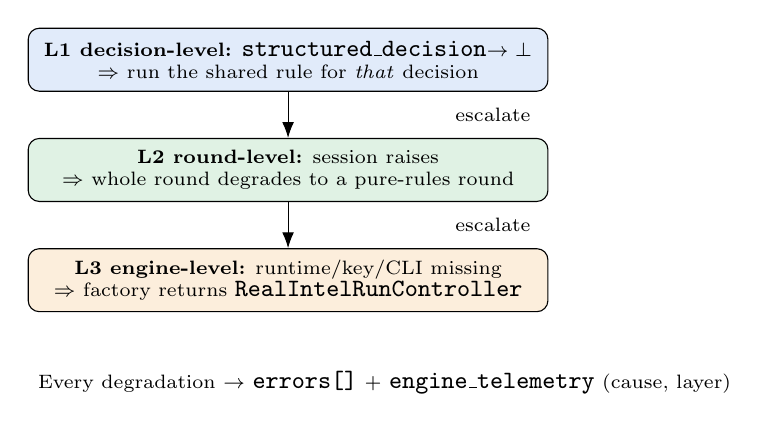
\begin{tikzpicture}[
  font=\scriptsize,
  lvl/.style={draw, rounded corners, align=center, minimum width=66mm, minimum height=8mm, inner sep=3pt},
  >={Latex[length=2mm]}
]
\node[lvl, fill=boxblue] (l1) at (0,2.0) {\textbf{L1 decision-level:} \code{structured\_decision}$\to\bot$\\$\Rightarrow$ run the shared rule for \emph{that} decision};
\node[lvl, fill=boxgreen] (l2) at (0,0.6) {\textbf{L2 round-level:} session raises\\$\Rightarrow$ whole round degrades to a pure-rules round};
\node[lvl, fill=boxorange] (l3) at (0,-0.8) {\textbf{L3 engine-level:} runtime/key/CLI missing\\$\Rightarrow$ factory returns \code{RealIntelRunController}};
\draw[->] (l1) -- (l2) node[midway,right,xshift=20mm]{escalate};
\draw[->] (l2) -- (l3) node[midway,right,xshift=20mm]{escalate};
\node[align=left, anchor=west] at (-3.3,-2.1) {Every degradation $\to$ \code{errors[]} + \code{engine\_telemetry} (cause, layer)};
\end{tikzpicture}
\caption{Three-layer fallback. Each layer degrades to the shared deterministic rules at a coarser granularity, and---unlike the prior design---records the cause and layer so degradation is observable, not silent.}
\label{fig:fallback}
\end{figure}

Reliability rests on three nested fallbacks, shown in Figure~\ref{fig:fallback}, all degrading to the \emph{same} \code{intel/rules.py} implementation so the two engines cannot drift:
\begin{itemize}
  \item \textbf{L1 (decision):} a failed structured decision returns \code{None}; the caller runs the rule for that one decision and the round continues.
  \item \textbf{L2 (round):} an exception anywhere in a round is caught and the round re-runs as a pure-rules round; the run does not abort.
  \item \textbf{L3 (engine):} if the SDK runtime, provider key, or bundled CLI is unavailable, the factory never constructs the agentic engine at all.
\end{itemize}
The key departure from the baseline is observability: every fallback appends an \code{ErrorRecord} and updates \code{engine\_telemetry} with the decision name, layer, and cause, so the structured-decision success rate and per-layer fallback rates become first-class evaluation metrics rather than invisible degradations.

\subsection{Budget and de-duplication hooks}

Budget enforcement lives in the local Python process, not the endpoint, via SDK \code{PreToolUse}/\code{PostToolUse} hooks. \code{PreToolUse} denies a source call when the run or per-round call cap is reached, or when the exact query was already executed, returning an instruction to the agent to change the query rather than failing silently; \code{PostToolUse} increments counters and records the call for blackboard accounting and bandit updates. Because hooks run locally they are the most reliable control point and do not depend on any endpoint capability.

\subsection{Provider portability}

The runtime targets Anthropic-\emph{compatible} endpoints rather than a single hosted model. A provider abstraction selects DeepSeek (\code{deepseek-v4-pro}/\code{-flash}) or GLM by environment variable, with an explicit \code{ANTHROPIC\_BASE\_URL}/\code{AUTH\_TOKEN} override, and maps a main and a fast model tier used respectively for planning and for the cheaper termination/relevance calls. All SDK imports are lazy so the package---and the rules engine---function without the agent dependency installed.

\section{Evaluation}
\label{sec:eval}

We designed the evaluation to make ``the agent is more intelligent'' a falsifiable, same-budget claim rather than a qualitative impression.

\subsection{Protocol}

Nine collection goals are frozen as a benchmark set: seven single-topic or broad goals---\emph{prompt-injection} (PI), \emph{jailbreak} (JB), \emph{RAG poisoning} (RAG), \emph{agent tool abuse} (ATA), \emph{model supply chain} (MSC), \emph{data leakage} (DL), and a six-topic \emph{broad LLM-security} sweep (BROAD)---plus two \emph{multi-topic} goals added to make coverage non-trivial to satisfy: \emph{IJA} (injection $+$ jailbreak $+$ agent-tool-abuse) and \emph{SRD} (supply-chain $+$ RAG $+$ data-leakage). For each goal we run the \code{rules} and \code{sdk} engines under identical safety valves (max API calls, max rounds) and repeat each three times on live sources. The \emph{primary} metric is \code{coverage\_completeness}---the fraction of target topics reaching the depth quota $q=3$ (Section~\ref{sec:termination})---computed engine-agnostically from the persisted blackboard. Secondary metrics are \emph{efficiency} (deduplicated relevant items per API call), the per-round \emph{marginal information} $g_t$, \emph{volume} (items per call), \emph{termination quality} (deviation between the actual stop round and the hindsight-optimal stop, the last round whose new-item yield exceeds 20\% of the run's peak), \emph{reliability} (structured-decision success and fallback rates), and \emph{cost} (wall-clock). An item counts as relevant if its three-tier verdict is \emph{relevant} or its rule score $\ge 0.68$. To keep the three repeats independent, each \code{sdk} run is given a cold-start bandit so persistent state does not leak across repeats.

\begin{table*}[t]
\centering
\caption{Same-budget A/B results across nine frozen goals (mean of three runs each; R = deterministic \code{rules}, S = agentic \code{sdk}). \textbf{Coverage completeness} (depth quota $q=3$) is the primary metric. The \code{sdk} engine is never below the baseline on coverage and far above it on the hard and multi-topic goals, trading per-call efficiency for that completeness. Bold marks the better engine where the gap is material.}
\label{tab:ab}
\renewcommand{\arraystretch}{1.15}
\setlength{\tabcolsep}{4.5pt}
\begin{tabular}{@{}l cc c cc c cc c cc c cc@{}}
\toprule
& \multicolumn{2}{c}{\textbf{Coverage}} && \multicolumn{2}{c}{\textbf{Relevant/call}} && \multicolumn{2}{c}{\textbf{Items/call}} && \multicolumn{2}{c}{\textbf{Topics}} && \multicolumn{2}{c}{\textbf{Rounds}} \\
\cmidrule{2-3}\cmidrule{5-6}\cmidrule{8-9}\cmidrule{11-12}\cmidrule{14-15}
\textbf{Goal} & R & S && R & S && R & S && R & S && R & S \\
\midrule
PI    & 1.00 & 1.00 && 2.47 & \textbf{2.83} && 3.16 & \textbf{4.34} && 2.0 & \textbf{4.7} && 1.0 & 5.0 \\
JB    & 1.00 & 1.00 && 2.53 & \textbf{3.48} && 3.16 & \textbf{6.41} && 3.0 & \textbf{4.0} && 1.0 & 5.3 \\
RAG   & 0.50 & \textbf{1.00} && \textbf{2.53} & 1.88 && 3.16 & \textbf{4.75} && 3.0 & \textbf{5.0} && 1.0 & 4.7 \\
ATA   & 0.00 & \textbf{1.00} && \textbf{3.22} & 1.96 && 4.15 & \textbf{6.62} && 4.0 & \textbf{5.3} && 5.0 & 3.7 \\
MSC   & 1.00 & 1.00 && \textbf{2.32} & 1.93 && 3.16 & \textbf{5.73} && \textbf{4.0} & 3.0 && 1.0 & 3.3 \\
DL    & 1.00 & 1.00 && 1.53 & \textbf{3.20} && 3.16 & \textbf{7.76} && 2.0 & \textbf{4.3} && 1.0 & 2.7 \\
BROAD & 0.67 & \textbf{0.89} && \textbf{3.66} & 2.72 && 5.33 & \textbf{8.60} && 5.0 & \textbf{6.0} && 8.0 & 7.7 \\
IJA   & 0.67 & \textbf{0.89} && \textbf{4.27} & 3.16 && 6.02 & 5.87 && 4.0 & 4.3 && 8.0 & 5.0 \\
SRD   & 0.33 & \textbf{0.78} && \textbf{3.21} & 2.51 && 4.21 & \textbf{6.71} && 4.0 & \textbf{5.0} && 1.0 & 4.7 \\
\midrule
\textbf{Mean} & 0.69 & \textbf{0.95} && \textbf{2.86} & 2.63 && 3.95 & \textbf{6.31} && 3.4 & \textbf{4.6} && -- & -- \\
\bottomrule
\end{tabular}
\end{table*}

\subsection{Coverage is the headline; efficiency is the price}

Table~\ref{tab:ab} is the full result, and the primary metric tells a clear story (Figure~\ref{fig:bars}a). On depth-quota coverage completeness the agentic engine reaches $1.00$ on six of nine goals against four for the baseline, is \emph{never} lower on any goal, and lifts the mean from $0.69$ to $0.95$ ($+38\%$). The gap is widest exactly where it matters: on agent-tool-abuse the deterministic templates reach the sparse target topic to quota \emph{never} ($0.00$) while the agent reaches it every time ($1.00$); on RAG, $0.50\!\to\!1.00$; and on the two multi-topic goals, $0.67\!\to\!0.89$ (IJA) and $0.33\!\to\!0.78$ (SRD).

That completeness has a price, and we report it plainly (Figure~\ref{fig:bars}b). On raw relevant-items-per-call the agent wins on PI, JB, and DL (the last by $+109\%$), but \emph{loses} on the goals where the coverage gate forces it to keep chasing a sparse topic (RAG $-26\%$, ATA $-39\%$, MSC $-17\%$, BROAD/IJA/SRD $-22$ to $-26\%$); averaged over goals it is $8\%$ \emph{lower}. The mechanism is visible in the same table: the agent retrieves $60\%$ more items per call and runs more rounds, because reaching a rare topic means issuing more, broader queries whose marginal items are individually less likely to clear the relevance bar. Figure~\ref{fig:tradeoff} makes the trade explicit: under the agent every goal moves \emph{rightward} toward full coverage, and the per-call efficiency moves up or down depending on how sparse the remaining topics are.

\begin{figure}[t]
\centering
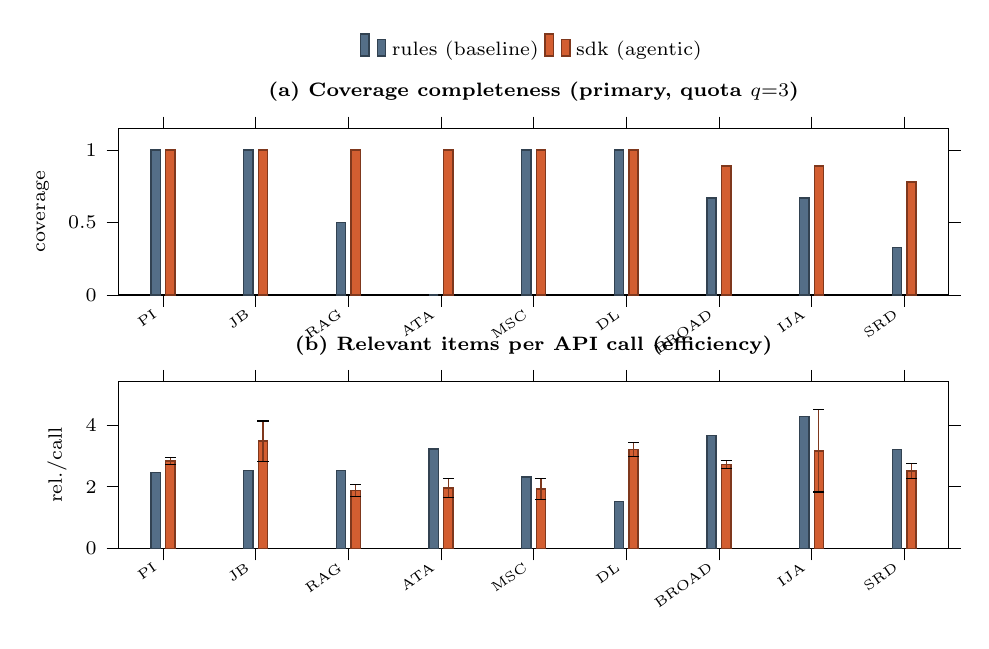
\begin{tikzpicture}
\begin{groupplot}[
  group style={group size=1 by 2, vertical sep=11mm},
  width=\columnwidth, height=3.7cm,
  symbolic x coords={PI,JB,RAG,ATA,MSC,DL,BROAD,IJA,SRD},
  xtick=data, ybar, /pgf/bar width=3.3pt,
  enlarge x limits=0.06, ymin=0,
  x tick label style={font=\tiny, rotate=35, anchor=east},
]
\nextgroupplot[title={(a) Coverage completeness (primary, quota $q{=}3$)},
  ylabel={coverage}, ymax=1.15, ytick={0,0.5,1},
  legend style={at={(0.5,1.34)}, anchor=south, legend columns=2}]
\addplot[fill=cRules, draw=cRules!60!black] coordinates {
  (PI,1) (JB,1) (RAG,0.5) (ATA,0) (MSC,1) (DL,1) (BROAD,0.67) (IJA,0.67) (SRD,0.33)};
\addlegendentry{rules (baseline)}
\addplot[fill=cSdk, draw=cSdk!60!black] coordinates {
  (PI,1) (JB,1) (RAG,1) (ATA,1) (MSC,1) (DL,1) (BROAD,0.89) (IJA,0.89) (SRD,0.78)};
\addlegendentry{sdk (agentic)}
\nextgroupplot[title={(b) Relevant items per API call (efficiency)},
  ylabel={rel./call}, ymax=5.4,
  error bars/y dir=both, error bars/y explicit]
\addplot[fill=cRules, draw=cRules!60!black] coordinates {
  (PI,2.47) (JB,2.53) (RAG,2.53) (ATA,3.22) (MSC,2.32) (DL,1.53) (BROAD,3.66) (IJA,4.27) (SRD,3.21)};
\addplot[fill=cSdk, draw=cSdk!60!black] coordinates {
  (PI,2.83)+-(0,0.12) (JB,3.48)+-(0,0.65) (RAG,1.88)+-(0,0.19)
  (ATA,1.96)+-(0,0.30) (MSC,1.93)+-(0,0.35) (DL,3.20)+-(0,0.23)
  (BROAD,2.72)+-(0,0.12) (IJA,3.16)+-(0,1.33) (SRD,2.51)+-(0,0.25)};
\end{groupplot}
\end{tikzpicture}
\caption{Same-budget comparison per goal. (a) Coverage completeness, the primary objective: the agent matches or exceeds the baseline everywhere and closes the gaps the fixed policy cannot (ATA $0.00\!\to\!1.00$). (b) Per-call efficiency is the price paid for that coverage---higher on PI/JB/DL, lower where sparse topics must be chased. Error bars: $\pm 1$ s.d.\ over three runs (the deterministic baseline is exactly reproducible, zero variance).}
\label{fig:bars}
\end{figure}

\begin{figure}[t]
\centering
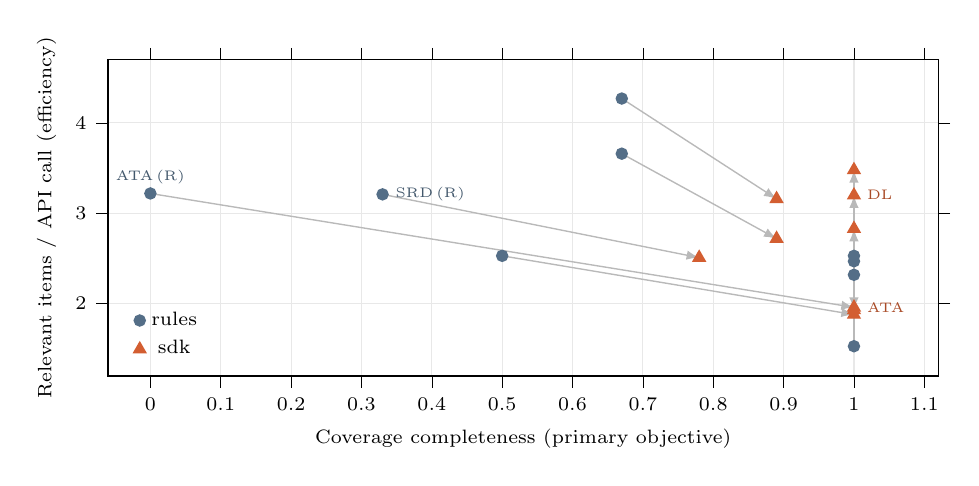
\begin{tikzpicture}
\begin{axis}[
  width=\columnwidth, height=5.6cm,
  xlabel={Coverage completeness (primary objective)},
  ylabel={Relevant items / API call (efficiency)},
  xmin=-0.06, xmax=1.12, ymin=1.2, ymax=4.7,
  grid=major, grid style={gray!18},
  legend style={at={(0.02,0.02)}, anchor=south west, legend columns=1},
]
% arrows rules -> sdk per goal
\draw[-{Latex[length=1.6mm]}, gray!55, line width=0.5pt] (axis cs:1,2.47) -- (axis cs:1,2.83);
\draw[-{Latex[length=1.6mm]}, gray!55, line width=0.5pt] (axis cs:1,2.53) -- (axis cs:1,3.48);
\draw[-{Latex[length=1.6mm]}, gray!55, line width=0.5pt] (axis cs:0.5,2.53) -- (axis cs:1,1.88);
\draw[-{Latex[length=1.6mm]}, gray!55, line width=0.5pt] (axis cs:0,3.22) -- (axis cs:1,1.96);
\draw[-{Latex[length=1.6mm]}, gray!55, line width=0.5pt] (axis cs:1,2.32) -- (axis cs:1,1.93);
\draw[-{Latex[length=1.6mm]}, gray!55, line width=0.5pt] (axis cs:1,1.53) -- (axis cs:1,3.20);
\draw[-{Latex[length=1.6mm]}, gray!55, line width=0.5pt] (axis cs:0.67,3.66) -- (axis cs:0.89,2.72);
\draw[-{Latex[length=1.6mm]}, gray!55, line width=0.5pt] (axis cs:0.67,4.27) -- (axis cs:0.89,3.16);
\draw[-{Latex[length=1.6mm]}, gray!55, line width=0.5pt] (axis cs:0.33,3.21) -- (axis cs:0.78,2.51);
\addplot[only marks, mark=*, mark size=2.0pt, color=cRules] coordinates {
  (1,2.47) (1,2.53) (0.5,2.53) (0,3.22) (1,2.32) (1,1.53) (0.67,3.66) (0.67,4.27) (0.33,3.21)};
\addlegendentry{rules}
\addplot[only marks, mark=triangle*, mark size=2.5pt, color=cSdk] coordinates {
  (1,2.83) (1,3.48) (1,1.88) (1,1.96) (1,1.93) (1,3.20) (0.89,2.72) (0.89,3.16) (0.78,2.51)};
\addlegendentry{sdk}
\node[font=\tiny, color=cRules!80!black, anchor=south] at (axis cs:0,3.22) {ATA\,(R)};
\node[font=\tiny, color=cRules!80!black, anchor=west] at (axis cs:0.33,3.21) {\,SRD\,(R)};
\node[font=\tiny, color=cSdk!80!black, anchor=west] at (axis cs:1,1.96) {\,ATA};
\node[font=\tiny, color=cSdk!80!black, anchor=west] at (axis cs:1,3.20) {\,DL};
\end{axis}
\end{tikzpicture}
\caption{Coverage--efficiency trade-off. Each arrow runs from a goal's deterministic point to its agentic point. Every goal moves \emph{rightward} to higher coverage (the sparse-topic goals ATA and SRD travel furthest, from $0.0$/$0.33$ to $1.0$/$0.78$); per-call efficiency rises or falls depending on how sparse the topics it must still reach are.}
\label{fig:tradeoff}
\end{figure}

\subsection{Why per-call efficiency is the wrong sole yardstick}

The agent-tool-abuse goal is the cleanest illustration. There the deterministic baseline posts one of the highest efficiencies in the study ($3.22$ rel./call)---yet its coverage completeness is $0.00$: its fixed keyword templates and round-robin never surface that sparse class to quota, so it efficiently re-collects easier topics and exhausts its rounds without ever covering the goal's namesake. The agent's $1.96$ rel./call looks worse only because it actually spends calls reaching the rare topic, which it covers fully ($1.00$). The baseline's apparent efficiency lead is thus an artifact of \emph{efficiently collecting the wrong thing}. The same pattern holds on the multi-topic goals SRD ($0.33\!\to\!0.78$) and IJA ($0.67\!\to\!0.89$) and on BROAD ($0.67\!\to\!0.89$): the coverage gate keeps the agent working the under-covered topic until quota or budget, which is exactly the behavior the stated objective demands. Across all goals the agent covers $+34\%$ more distinct topics and retrieves $+60\%$ more items per call (Table~\ref{tab:ab}), the latter a direct consequence of its heavier, agent-chosen use of advanced operators.

\subsection{The marginal-information signal and cheap adjudication}

The three-tier cascade keeps relevance annotation nearly free: across all agentic runs the embedding tier adjudicated $3{,}256$ items while the costly flash-LLM tier was invoked on only $70$ ($\approx 1\%$), the remainder resolved by the zero-cost rule tier. Those same labels feed the per-round marginal-information signal $g_t$ that the termination ladder watches. Figure~\ref{fig:infogain} plots $g_t$ over rounds for three representative runs: it starts high and decays unevenly as a goal's easy items are exhausted, with transient rebounds when the agent reformulates onto a fresh sub-topic. The stall floor $\tau=0.5$ is drawn dashed; in this benchmark no run's $g_t$ stayed below it for the two-round patience window, so the stall valve never fired (Section~\ref{sec:term-result}) and runs ended by coverage completion or the round cap first. The signal is nonetheless the safety mechanism that bounds the coverage gate when a sparse topic is genuinely unreachable.

\begin{figure}[t]
\centering
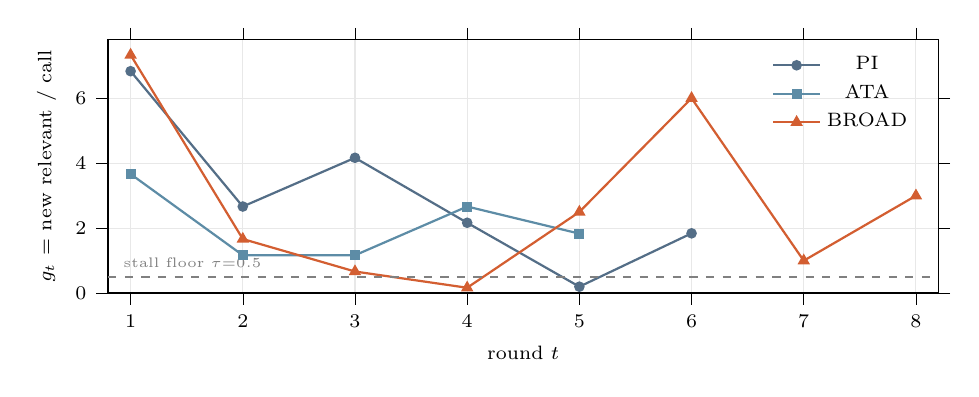
\begin{tikzpicture}
\begin{axis}[
  width=\columnwidth, height=4.8cm,
  xlabel={round $t$}, ylabel={$g_t$ = new relevant / call},
  xmin=0.8, xmax=8.2, ymin=0, ymax=7.8,
  xtick={1,2,3,4,5,6,7,8},
  grid=major, grid style={gray!18},
  legend style={at={(0.98,0.98)}, anchor=north east, legend columns=1},
]
\addplot[mark=*, mark size=1.5pt, color=cRules, thick] coordinates {
  (1,6.833) (2,2.667) (3,4.167) (4,2.167) (5,0.2) (6,1.842)};
\addlegendentry{PI}
\addplot[mark=square*, mark size=1.4pt, color=cTier2, thick] coordinates {
  (1,3.667) (2,1.167) (3,1.167) (4,2.667) (5,1.833)};
\addlegendentry{ATA}
\addplot[mark=triangle*, mark size=1.8pt, color=cSdk, thick] coordinates {
  (1,7.333) (2,1.667) (3,0.667) (4,0.167) (5,2.5) (6,6.0) (7,1.0) (8,3.0)};
\addlegendentry{BROAD}
\addplot[dashed, gray, line width=0.6pt] coordinates {(0.8,0.5) (8.2,0.5)};
\node[font=\tiny, gray, anchor=south west] at (axis cs:0.85,0.5) {stall floor $\tau{=}0.5$};
\end{axis}
\end{tikzpicture}
\caption{The marginal-information signal $g_t$ (new relevant items per API call) per round for three representative agentic runs. It decays unevenly with reformulation rebounds; the stall valve stops a run only if $g_t$ stays below $\tau$ for the patience window, which never occurs here---coverage or the round cap ends runs first.}
\label{fig:infogain}
\end{figure}

\subsection{Termination, reliability, and cost}
\label{sec:term-result}

On \emph{termination quality} the agent is cleanly better: its stop round matched the hindsight-optimal round on all nine goals (mean deviation $0.0$), whereas the deterministic stop condition overshot (mean deviation $0.22$, e.g.\ a round late on BROAD)---its rule cannot read a yield plateau. The stall valve was available on every run but never triggered (stall rate $0$ on all goals): the marginal-information signal never stayed below $\tau$ for the patience window before either coverage completed or the round cap intervened, so the valve served purely as the latent guard it is designed to be. On \emph{reliability}, across $436$ live structured decisions the engine recorded a $97.7\%$ success rate ($426/436$) with a $2.3\%$ fallback rate, every fallback logged with its layer and cause; no run aborted. This confirms the endpoint capability spike, which had recorded $100\%$ tool-call (20/20) and structured-decision parse (20/20) reliability on the DeepSeek Anthropic-compatible endpoint, with native JSON-schema output and prompt caching unsupported---precisely why the architecture defaults to tool forcing and summary-based cost control. The \emph{cost} is the honest counterweight: agentic runs took roughly an order of magnitude more wall-clock ($\sim$20--112\,s for \code{rules}; $\sim$200--1950\,s for \code{sdk}), the price of an LLM in the loop, more rounds, and multi-round tool use.

Independently, the UCB1 source recommender was validated offline by replaying 33 historical runs (617 rounds): bandit regret $1.063$ versus round-robin regret $1.245$ (lower is better), confirming the recommender beats uniform polling with no API spend.

\subsection{Threats to validity}

Three caveats bound these claims. (i)~\emph{Relevance is heuristic}: the per-call ``relevant'' counts and the coverage assignment rest on the three-tier label, not human gold; a precision audit with two annotators and a cross-family LLM judge is the next step, and would firm up the efficiency comparison most. (ii)~\emph{Variance}: making completeness a hard constraint sharply reduced the agent's run-to-run spread relative to a yield-only stop---coverage standard deviation is $0$ on six of nine goals and $\le 0.19$ elsewhere, and efficiency s.d.\ is $\le 0.35$ rel./call on seven goals, with IJA the lone outlier ($\pm 1.33$); the deterministic baseline remains exactly reproducible. (iii)~\emph{Endpoint specificity}: results are for one provider (DeepSeek); the portability layer is in place but the GLM path is unmeasured here.

\section{Discussion, Limitations, and Future Work}

\textbf{When does autonomy pay?} The evaluation gives a concrete answer rather than a slogan. Autonomy pays when completeness matters and the goal contains a sparse or hard-to-phrase topic that fixed templates miss (ATA, SRD, IJA, BROAD): there the coverage gate plus the agent's freedom to reformulate queries close gaps the baseline cannot ($+38\%$ mean coverage; ATA $0.00\!\to\!1.00$), and coverage---not per-call efficiency---is the metric that moves. Autonomy is \emph{not} worth its cost when a goal is narrow, already reachable by a hand-tuned template, and judged only on per-call efficiency (RAG, MSC): the deterministic engine matches the agent's coverage at a fraction of the wall-clock. A practical deployment can therefore route by goal breadth, reserving the agentic engine for broad or sparse missions and the cheap deterministic engine for narrow ones---a routing the shared engine factory already makes a one-line choice.

\textbf{Why a hybrid, not a fully autonomous agent.} A fully agentic loop---the agent calling source tools directly until it decides to stop---is technically unlocked: the MCP tools and hooks are in place and live tool reliability was $97.7\%$. We nonetheless keep the controller authoritative over budget, coverage, and persistence, because an architecture whose worst case is a verified rule engine is safer to deploy and easier to evaluate than one whose worst case is an unbounded model; the order-of-magnitude cost gap also argues for keeping the loop bounded. Full autonomy remains gated on evidence, not capability.

\textbf{Limitations.} (i)~The relevance signal, though improved by the three-tier filter, remains heuristic, and it now also drives the coverage assignment; the precision audit (Section~\ref{sec:eval}, threats) is the highest-value next step and would most affect both the efficiency \emph{and} coverage comparisons. (ii)~The bandit's reward (new items per call) optimizes \emph{novelty}, which can under-weight a small number of high-value confirmations; a value-weighted reward is future work. (iii)~The agentic engine adds an LLM in the loop, costing roughly an order of magnitude more wall-clock; context discipline and fast-model termination mitigate but do not eliminate this. (iv)~Provider portability is validated mainly on one endpoint; the GLM path is retained as a fallback pending subscription renewal.

\textbf{Future work.} Beyond completing the A/B study, the natural next steps are a value-weighted bandit reward, a fully agentic mode behind the existing tools and hooks, and feeding the per-item relevance \code{method} labels back as supervision for the filter. The collected, relevance-annotated items are already the input corpus for a downstream knowledge-graph construction stage, which we treat as out of scope here.

\section{Conclusion}

We described the architecture of an autonomous LLM-security intelligence-collection agent built on a hybrid controller: an LLM reasons over a compact, persisted metric digest to make four decisions---source selection, query and operator formulation, rewrite, and termination---while a Python controller retains the loop, budget safety valves, accounting, and persistence. Termination is governed by a coverage-first policy: a depth-quota coverage gate makes completeness a hard constraint and a marginal-information stall detector guards against futile loops, with the LLM stop decision operating only inside that envelope. A shared deterministic rule module serves simultaneously as the baseline engine and as the per-decision, per-round, and per-engine fallback, so the system's floor is a verified rule-based collector and its degradations are observable rather than silent. A same-budget A/B study over nine frozen goals characterizes the outcome honestly: on the primary objective the agentic engine matches or exceeds the baseline's coverage on every goal and lifts the mean from $0.69$ to $0.95$ ($+38\%$), closing sparse gaps the fixed policy never reaches (agent-tool-abuse $0.00\!\to\!1.00$), while retrieving $+60\%$ more items per call and terminating at the hindsight-optimal round throughout, at $97.7\%$ live decision reliability. The price is per-call efficiency---$8\%$ lower on average and an order of magnitude more wall-clock---paid precisely where the agent chases topics the baseline abandons. The contribution is thus not only an architecture but a clear account of \emph{when} autonomy in intelligence collection earns its cost---when coverage completeness matters and topics are sparse---enabling a goal-aware choice between the two engines the design already unifies.

\bibliographystyle{IEEEtran}
\bibliography{references}

\end{document}
